% main.tex (Stage II Report)
\documentclass[12pt,a4paper]{report}
\usepackage[utf8]{inputenc}
\usepackage[T1]{fontenc}
\usepackage{times}
\usepackage{geometry}
\usepackage{setspace}
\usepackage{graphicx}
\usepackage{caption}
\usepackage{tikz}
\usetikzlibrary{calc, positioning, shapes.geometric, arrows.meta, fit, backgrounds}
\usepackage{ragged2e}
\usepackage{everypage}
\usepackage{etoolbox}
\usepackage{booktabs}
\usepackage{longtable}
\usepackage{enumitem}
\usepackage{hyperref}
\geometry{left=1in,right=1in,top=1in,bottom=1in}
\onehalfspacing
\pagestyle{plain}
\usepackage{fancyhdr}
\usepackage{titlesec}
\usepackage{float}
\usepackage{pgfplots}
\pgfplotsset{compat=1.18}
\usepackage{tocloft}

\usepackage[a4paper, top=0.9in, bottom=1in, left=1in, right=1in, headheight=15pt, headsep=3pt]{geometry}

% -----------------------
% Metadata
% -----------------------
\newcommand{\UniversityName}{Savitribai Phule Pune University}
\newcommand{\CollegeName}{Rajiv Gandhi College of Engineering}
\newcommand{\DepartmentName}{Department of Computer Engineering}
\newcommand{\LocationLine}{Karjule Harya, Tal. Parner, Dist. Ahilyanagar 414 304}
\newcommand{\AcademicYear}{2025-2026}
\newcommand{\ProjectTitle}{AI-POWERED DIET ASSISTANT}
\newcommand{\GuideName}{Prof. Rahinj P. L.}
\newcommand{\StudentOne}{Aher Dhiraj Ramchandra}
\newcommand{\StudentTwo}{Bhise Dhanashri Dnyaneshwar}
\newcommand{\StudentThree}{Adhav Gauri Janardhan}
\newcommand{\StudentFour}{Tejas Bhabad Dattatray}
\newcommand{\SeatOne}{72265280B}
\newcommand{\SeatTwo}{72265297G}
\newcommand{\SeatThree}{72265305M}
\newcommand{\SeatFour}{72339517K}

% Border control
\newbool{frontborder}
\booltrue{frontborder}

\AddEverypageHook{%
  \ifbool{frontborder}{%
    \begin{tikzpicture}[remember picture,overlay]
      \draw[line width=1pt]
        ($(current page.north west) + (8mm,-8mm)$) rectangle
        ($(current page.south east) + (-8mm,8mm)$);
    \end{tikzpicture}%
  }{}%
}

\begin{document}
\pagenumbering{roman}

% ============ TITLE PAGE ============
\begin{titlepage}
  \centering
  \vspace*{-4mm}
  {\normalsize \UniversityName\\[12pt]}
  {\normalsize\bfseries A PROJECT STAGE II REPORT\\[12pt] ON\\[24pt]
  \Large\textbf{“\ProjectTitle”}\\[24pt]}
  {\small SUBMITTED TO THE UNIVERSITY OF PUNE, PUNE\\
  IN PARTIAL FULFILLMENT OF THE REQUIREMENTS\\
  FOR THE AWARD OF THE DEGREE\\[6pt]
  \vspace{8mm}
  \textbf{BACHELOR OF ENGINEERING}\\(Computer Engineering)\\[14pt]}
  {\normalsize\bfseries BY\\[8pt]}
  \begin{center}
\begin{tabular}{l l}
\textbf{\StudentOne} & \textbf{Exam Seat No: \SeatOne} \\
\textbf{\StudentTwo} & \textbf{Exam Seat No: \SeatTwo} \\
\textbf{\StudentThree} & \textbf{Exam Seat No: \SeatThree} \\
\textbf{\StudentFour} & \textbf{Exam Seat No: \SeatFour} \\
\end{tabular}
\end{center}

  {\normalsize Under the Guidance of\\ \textbf{\GuideName}\\[18pt]}
  {\small\bfseries \DepartmentName\\ \CollegeName\\ \LocationLine\\[6pt]}
  {\small\bfseries \AcademicYear}
\end{titlepage}

% ============ CERTIFICATE ============
\newpage
\thispagestyle{plain}
\begin{center}
  {\large\bfseries \DepartmentName\\[1pt] \CollegeName\\[1pt] \LocationLine\\[12pt]}
  \vspace{6pt}
  {\Large \bfseries C E R T I F I C A T E}\\[8pt]
\end{center}

\noindent\centering This is to certify that the Stage II Report entitled
\begin{center}
  {\large\textbf{“\ProjectTitle”}}
\end{center}
\textbf{Submitted by}
\begin{center}
\begin{tabular}{l l}
\textbf{\StudentOne} & \textbf{Exam Seat No: \SeatOne} \\
\textbf{\StudentTwo} & \textbf{Exam Seat No: \SeatTwo} \\
\textbf{\StudentThree} & \textbf{Exam Seat No: \SeatThree} \\
\textbf{\StudentFour} & \textbf{Exam Seat No: \SeatFour} \\
\end{tabular}
\end{center}
are bonafide students of this institute and the work has been carried out by them under the supervision of \textbf{\GuideName} and it is approved for the partial fulfillment of the requirement of Savitribai Phule Pune University, for the award of the degree of Bachelor of Engineering (Computer Engineering).

\vspace{12pt}
\noindent
\begin{minipage}[t]{0.46\textwidth}
  \textbf{Place:}\\[4pt]
  \textbf{Date:}\\[4pt]
\end{minipage}
\hfill
\vspace{8mm}

\begin{center}
  \begin{tabular*}{0.92\textwidth}{@{\extracolsep{\fill}} c c}
    \begin{tabular}{c}
      \textbf{\GuideName}\\[-2pt]
      \textbf{Internal Guide}\\[-2pt]
      \textbf{Dept. of Computer Engg.}
    \end{tabular}
    &
    \begin{tabular}{c}
      \textbf{Project Coordinator Name}\\[-2pt]
      \textbf{Project Coordinator}\\[-2pt]
      \textbf{Dept. of Computer Engg.}
    \end{tabular}
  \end{tabular*}

  \vspace{1.2cm}

  \begin{tabular*}{0.92\textwidth}{@{\extracolsep{\fill}} c c}
    \begin{tabular}{c}
      \textbf{Prof. Examiner Name}\\[-2pt]
      \textbf{Internal Examiner}\\[-2pt]
      \textbf{Dept. of Computer Engg.}
    \end{tabular}
    &
    \begin{tabular}{c}
      \textbf{HOD Name}\\[-2pt]
      \textbf{H.O.D.}\\[-2pt]
      \textbf{Dept. of Computer Engg.}
    \end{tabular}
  \end{tabular*}

  \vspace{1.2cm}

  \begin{tabular*}{0.92\textwidth}{@{\extracolsep{\fill}} c c}
    \begin{tabular}{c}
      \textbf{External Examiner Name}\\[-2pt]
      \textbf{External Examiner}
    \end{tabular}
    &
    \begin{tabular}{c}
      \textbf{Principal Name}\\[-2pt]
      \textbf{Principal}\\[-2pt]
      \textbf{RGCOE, Karjule Harya}
    \end{tabular}
  \end{tabular*}
\end{center}

% ============ CERTIFICATE BY GUIDE ============
\newpage
\thispagestyle{plain}
\begin{center}
  {\Large \bfseries CERTIFICATE BY GUIDE}\\[16pt]
\end{center}
\justifying
This is to certify that \textbf{\StudentOne}, \textbf{\StudentTwo}, \textbf{\StudentThree}, and \textbf{\StudentFour} have completed the Project Stage II work under my guidance and supervision and that I have verified the work for its originality in documentation, problem statement, and results presented in this stage. Any reproduction of other necessary work is with prior permission, and due ownership has been acknowledged and included in the references.

\vspace{12pt}
\noindent
\begin{minipage}[t]{0.46\textwidth}
  \textbf{Place:}\\[4pt]
  \textbf{Date:}\\[4pt]
\end{minipage}
\hfill
\begin{minipage}[t]{0.46\textwidth}
  \centering
  \textbf{\GuideName}\\[-2pt]
  \textbf{Project Guide}
\end{minipage}

% ============ ACKNOWLEDGEMENT ============
\newpage
\section*{\centering ACKNOWLEDGEMENT}
\addcontentsline{toc}{chapter}{Acknowledgement}
\vspace{8mm}
\justifying

We would like to express our sincere gratitude to all those who helped us in the successful completion of our Project Stage-II Report on ``\textbf{AI-POWERED DIET ASSISTANT}''.

We are highly thankful to our Project Guide, \textbf{\GuideName}, for his valuable guidance, encouragement, and continuous support throughout the project work.

We express our gratitude to our Project Coordinator, \textbf{Prof. Coordinator Name}, for his/her guidance and support. We are also thankful to \textbf{Prof. Rahinj P. L.}, Head of the Department of Computer Engineering, for providing the necessary facilities and encouragement.

We extend our sincere thanks to \textbf{Prof. Vice Principal Name}, Vice Principal, and \textbf{Prof. Pawar K. P.}, Principal of RGCOE, for their motivation and support.

We also thank all the teaching and non-teaching staff members of the Department of Computer Engineering for their cooperation and assistance.

Finally, we express our heartfelt gratitude to our family, friends, and everyone who directly or indirectly contributed to the successful completion of this project.

\vspace{15mm}

\begin{flushright}
\textbf{\StudentOne}\\
\textbf{\StudentTwo}\\
\textbf{\StudentThree}\\
\textbf{\StudentFour}
\end{flushright}

% ============ ABSTRACT ============
\newpage
\section*{\centering ABSTRACT}
\addcontentsline{toc}{chapter}{Abstract}
\vspace{8mm}
\justifying

The increasing prevalence of lifestyle-related diseases established an urgent need for effective, user-friendly dietary monitoring tools. Traditional nutrition tracking applications demanded tedious manual entry, precise ingredient measurements, and rigid database lookups, which significantly reduced long-term user engagement and consistency. To solve this issue, we developed NutiAI, an intelligent dietary tracking system that leveraged Large Language Models (LLMs) to automatically extract exact nutritional content directly from natural conversational text. The system was implemented using a modern full-stack architecture, featuring a React-based frontend for a premium user interface and a Node.js backend integrated with a MySQL database via Drizzle ORM for secure data management. By utilizing advanced Natural Language Processing (NLP) through the Google Gemini API and local Ollama models, the application successfully parsed unstructured meal descriptions into accurate caloric and macronutrient data in real time. The results demonstrated that conversational food logging, coupled with gamified health scores and multilingual support across English, Hindi, and Spanish, drastically improved user interaction and broadened accessibility. Ultimately, NutiAI modernized nutritional management by offering a highly inclusive and scalable framework that simplified diet tracking and promoted sustainable health habits. Future extensions of this work could involve integration with IoT wearable devices and the implementation of predictive health analytics for proactive wellness management.

\vspace{12pt}

\noindent \textbf{Keywords:} Artificial Intelligence, Large Language Models, Natural Language Processing, Nutrition Tracking, Gamification, Full-Stack Development.

% ============ SYNOPSIS ============
\newpage
\section*{\centering SYNOPSIS}
\addcontentsline{toc}{chapter}{Synopsis}
\vspace{8mm}
\justifying

\subsection*{1. Title Page Information}
\textbf{Project Title:} AI-POWERED DIET ASSISTANT\\[4pt]
\textbf{Team Members:}\\
1. Aher Dhiraj Ramchandra (Seat No: 72265280B)\\
2. Bhise Dhanashri Dnyaneshwar (Seat No: 72265297G)\\
3. Adhav Gauri Janardhan (Seat No: 72265305M)\\
4. Tejas Bhabad Dattatray (Seat No: 72339517K)\\[4pt]
\textbf{Guide:} Prof. Rahinj P. L.\\[4pt]
\textbf{Department \& College:} Department of Computer Engineering, Rajiv Gandhi College of Engineering

\subsection*{2. Abstract}
The increasing prevalence of lifestyle-related diseases established an urgent need for effective, user-friendly dietary monitoring tools. Traditional nutrition tracking applications demanded tedious manual entry, precise ingredient measurements, and rigid database lookups, which significantly reduced long-term user engagement and consistency. To solve this issue, we developed NutiAI, an intelligent dietary tracking system that leveraged Large Language Models (LLMs) to automatically extract exact nutritional content directly from natural conversational text. The system was implemented using a modern full-stack architecture, featuring a React-based frontend for a premium user interface and a Node.js backend integrated with a MySQL database via Drizzle ORM for secure data management. By utilizing advanced Natural Language Processing (NLP) through the Google Gemini API and local Ollama models, the application successfully parsed unstructured meal descriptions into accurate caloric and macronutrient data in real time. The results demonstrated that conversational food logging, coupled with gamified health scores and multilingual support across English, Hindi, and Spanish, drastically improved user interaction and broadened accessibility. Ultimately, NutiAI modernized nutritional management by offering a highly inclusive and scalable framework that simplified diet tracking and promoted sustainable health habits. Future extensions of this work could involve integration with IoT wearable devices and the implementation of predictive health analytics for proactive wellness management.

\subsection*{3. Introduction / Background}
Traditional diet management relies heavily on strict manual logging, causing significant user fatigue. With the rapid evolution of conversational AI and Natural Language Processing (NLP), there is an unprecedented opportunity to simplify this process. NutiAI acts as an AI-powered diet assistant that understands conversational meal descriptions, autonomously calculates macros, and provides gamified feedback to encourage sustainable healthy habits.

\subsection*{4. Problem Statement}
Existing diet applications depend on rigid and tedious manual inputs, requiring users to weigh ingredients and search through vast localized databases. NutiAI addresses this limitation by using LLMs to process simple conversational text inputs (e.g., "I ate two scrambled eggs"), automatically estimating precise macronutrients and offering a premium, user-friendly multilingual experience.

\subsection*{5. Objectives}
\begin{itemize}[leftmargin=*]
    \item To develop an NLP-based system capable of extracting precise macronutrients from conversational text.
    \item To automatically assign health scores and estimate calories using Large Language Models.
    \item To create a personalized, interactive AI diet planning agent for real-time coaching.
    \item To deliver seamless multilingual support (English, Hindi, Spanish) for broader accessibility.
    \item To ensure highly secure data handling utilizing Node.js, MySQL, and Clerk Authentication.
\end{itemize}

\subsection*{6. Proposed System / Methodology}
The system is built on a modern, robust full-stack architecture. Users log their meals via a text-based conversational interface on a React frontend. The Node.js backend processes these requests by calling the Google Gemini API or a local Ollama model to accurately parse nutritional data. This structured data is securely stored in a MySQL database using Drizzle ORM and displayed to the user via premium, engaging dashboard animations.

\subsection*{7. Scope of the Project}
The project covers natural language food logging, real-time AI diet coaching, gamification of health scores, and dynamic multilingual localization. It focuses strictly on dietary tracking and does not currently encompass clinical medical diagnostics or real-time IoT wearable sensor tracking.

\subsection*{8. Applications / Use Cases}
\begin{itemize}[leftmargin=*]
    \item Personal dietary and calorie tracking via simple conversational input.
    \item Multilingual health coaching for diverse, non-English speaking demographics.
    \item Gamified fitness planning and tracking for health enthusiasts.
\end{itemize}

\subsection*{9. Software \& Hardware Requirements}
\begin{itemize}[leftmargin=*]
    \item \textbf{Software:} Node.js (v18+), React (Vite), Tailwind CSS, MySQL, Drizzle ORM.
    \item \textbf{Hardware:} Minimum Intel i3/i5 processor, 8GB RAM, and a stable internet connection.
\end{itemize}

\subsection*{10. Conclusion}
NutiAI significantly reduces the inherent friction of diet tracking by introducing an intuitive, AI-driven, and multilingual interface. By shifting the burden of calculation from the user to the AI, it promotes long-term adherence to healthier lifestyles.

\subsection*{11. References}
\begin{itemize}[leftmargin=*]
    \item [1] A. Vaswani et al., "Attention is All You Need," \textit{Advances in Neural Information Processing Systems}, 2017.
    \item [2] Google DeepMind, "Gemini: A Family of Highly Capable Multimodal Models," 2023.
    \item [3] S. Ghosh and S. Sahu, "AI-Based Diet Recommendation Systems: A Review," \textit{Int. J. Adv. Comput. Sci. Appl.}, 2021.
\end{itemize}


% ============ ABBREVIATIONS ============
\newpage
\section*{\centering Abbreviations}
\addcontentsline{toc}{chapter}{Abbreviations}

\textbf{Purpose} \\
The \textit{Abbreviations} section lists all short forms and their full meanings used in the report. For example, AI stands for Artificial Intelligence.

\textbf{Placement} \\
Usually comes before the \textit{Introduction} section.

\textbf{Format}
\begin{itemize}
    \item Arranged alphabetically (A $\rightarrow$ Z).
    \item Keeps consistency across the report.
\end{itemize}

\vspace{5mm}

\begin{description}[leftmargin=3cm,style=nextline]
  \item[AI] Artificial Intelligence
  \item[API] Application Programming Interface
  \item[CNN] Convolutional Neural Network
  \item[DBMS] Database Management System
  \item[GUI] Graphical User Interface
  \item[HTTP] Hypertext Transfer Protocol
  \item[IoT] Internet of Things
  \item[JSON] JavaScript Object Notation
  \item[JWT] JSON Web Token
  \item[LLM] Large Language Model
  \item[ML] Machine Learning
  \item[NLP] Natural Language Processing
  \item[ORM] Object-Relational Mapping
  \item[RAM] Random Access Memory
  \item[REST] Representational State Transfer
  \item[SQL] Structured Query Language
  \item[UI] User Interface
  \item[UX] User Experience
\end{description}

% ============ TABLE OF CONTENTS ============
\newpage
\tableofcontents

% ============ LIST OF FIGURES ============
\newpage
\listoffigures
\addcontentsline{toc}{chapter}{List of Figures}

% ============ LIST OF TABLES ============
\newpage
\listoftables
\addcontentsline{toc}{chapter}{List of Tables}


% =========================================
% CHAPTER 1: INTRODUCTION
% =========================================
\newpage
\pagenumbering{arabic}
\thispagestyle{fancy}

\chapter{Introduction} 

\section{Introduction}
The rapid advancement of modern technologies such as Artificial Intelligence (AI), Large Language Models (LLMs), and Web Development has significantly transformed various sectors by providing intelligent and automated solutions. In the domain of healthcare and personal wellness, consistent dietary tracking remains a cornerstone of long-term health management. However, traditional dietary tracking methods require tedious manual data entry, leading to high user drop-off rates and inconsistent nutritional monitoring. 

The proposed NutiAI project aims to develop an effective solution for the identified problem of manual dietary tracking using modern technologies and engineering principles. NutiAI is an intelligent web application that parses conversational meal descriptions to extract precise macronutrients and calories in real time. By leveraging natural language processing, NutiAI overcomes the friction and cognitive load of manually searching, measuring, and logging daily nutritional intake, promoting accessible health management for diverse demographics.

\section{Motivation of the Project}
The motivation behind this project is to overcome the limitations of existing systems and provide a smart, efficient, and reliable solution. Traditional health logging applications rely heavily on complex user interfaces and the manual labor required to log individual meal components. This creates significant friction and user fatigue, discouraging consistent tracking.

The NutiAI project was selected to eliminate these barriers by making diet tracking as simple as sending a text message. By shifting the burden of calorie calculation and portion estimation from the user to intelligent Large Language Models, this project bridges the gap between advanced generative AI and everyday wellness. The expected benefits include increased user retention, precise macronutrient tracking without rigid database lookups, and multilingual accessibility that caters to a broader global audience.

\section{Aim and Objectives}

\subsection{Aim}
To design and develop an intelligent, efficient, and reliable conversational diet tracking system that simplifies nutritional monitoring using Large Language Models.

\subsection{Objectives}
\begin{itemize}[leftmargin=*]
    \item To successfully parse complex, natural language meal descriptions and return accurate nutritional data within a response time of under 3 seconds.
    \item To integrate Google Gemini and local Ollama APIs with a secure Node.js backend and a responsive React frontend.
    \item To implement real-time gamified health scoring to encourage user consistency.
    \item To deliver seamless multilingual support across English, Hindi, and Spanish to ensure broader accessibility.
\end{itemize}

\section{Problem Statement}
Health-conscious individuals, fitness enthusiasts, and people with specific dietary goals frequently struggle with tracking consistency. The core problem lies in the repetitive and tedious task of measuring ingredients and searching for precise food items in traditional applications. Current diet trackers rely on rigid, localized SQL databases that cannot understand conversational context or mixed meals, requiring users to manually log every component. 

This friction leads to high drop-off rates and incomplete nutritional data. There is a critical need for a frictionless logging method that drastically reduces logging time, provides automated portion estimation, and allows intuitive natural language interactions to maintain long-term user engagement.

\section{Existing System}
The existing system performs operations using conventional methods and available technologies. Widely used applications, such as MyFitnessPal or traditional calorie counters, require users to manually input food weight and select items from rigid drop-down menus or by scanning barcodes. These platforms utilize traditional relational databases and static search algorithms. While these systems can be highly accurate when users perfectly measure and log every single ingredient, they completely lack the ability to process conversational input or understand unstructured text.

\section{Limitations of Existing System}
\begin{itemize}[leftmargin=*]
    \item \textbf{High manual dependency:} Users must manually search for and log every individual ingredient.
    \item \textbf{Inflexibility:} Complete inability to parse unstructured or conversational text inputs.
    \item \textbf{Performance limitations:} Time-consuming for users to log complex, multi-ingredient meals, leading to application abandonment.
    \item \textbf{Maintenance overhead:} A constant need to manually update local food databases with new items.
    \item \textbf{Lack of automation:} The burden of calculation and portion estimation falls entirely on the user.
\end{itemize}

\section{Proposed System}
The proposed system, NutiAI, is designed to overcome the limitations of the existing system through automation, real-time monitoring, and intelligent processing. NutiAI utilizes a modern full-stack architecture comprising a React frontend, a Node.js/Express backend, and a MySQL database managed by Drizzle ORM. 

When a user inputs a conversational meal description (e.g., "I had two scrambled eggs and a piece of toast"), the backend queries an LLM API (such as Gemini or Ollama) with a specialized prompt. The LLM processes the unstructured text and returns structured JSON data containing exact calories and macronutrients. This completely eliminates manual searching and measuring, offers instant gamified feedback, and supports multiple languages. By shifting the processing burden to the AI, NutiAI provides a highly scalable and frictionless dietary tracking experience.

% =========================================
% CHAPTER 2: LITERATURE SURVEY
% =========================================
\chapter{Literature Survey}

\section{Literature Survey}
The Literature Survey chapter provides a detailed review of previously published research papers, journals, conference papers, and technical articles related to the selected project domain. It helps in understanding the existing technologies, methodologies, algorithms, tools, and techniques used by different researchers to solve similar problems.

The purpose of conducting a literature survey is to identify the strengths and limitations of existing systems and to find research gaps that can be addressed in the proposed project. To build a robust foundation for NutiAI, a comprehensive review of recent breakthroughs in applied Natural Language Processing (NLP), Large Language Models (LLMs), and AI-based dietary tracking algorithms was conducted. Papers were sourced from authentic platforms such as IEEE, Springer, and recognized AI conferences, focusing primarily on developments between 2017 and 2023.

By evaluating different techniques for parsing unstructured text and comparing various generative AI models, the survey highlighted a clear paradigm shift from rigid database lookups to dynamic conversational intelligence. This research directly motivated the architecture of NutiAI, highlighting the need to overcome existing limitations such as high computational costs and the lack of real-time user gamification.

\section{Review of Related Work}
Vaswani et al. introduced the Transformer architecture, which serves as the foundational technology for modern sequence modeling and NLP tasks. The system achieved unprecedented accuracy in natural language understanding using attention mechanisms. However, the proposed approach originally required massive training datasets and faced challenges in real-time edge implementation due to higher computational requirements [1]. This foundational work enables the entity extraction utilized by NutiAI.

Google DeepMind developed highly capable Multimodal Models under the Gemini family. Their work improved the contextual understanding of unstructured data by applying large language models for complex reasoning. Their models successfully achieved cross-domain intelligence but suffered from API dependence and increased latency for offline edge deployment [2]. NutiAI leverages this reasoning capability to accurately parse complex meal descriptions into structured nutritional data.

Ghosh et al. implemented an AI-based diet recommendation system leveraging NLP and data analytics. The system provided accurate forecasting for dietary needs, but the model's user adherence decreased when lacking integration with real-time gamified interactions and modern frontend architectures [3]. This gap identified the crucial need for NutiAI to incorporate gamified health scoring and an engaging user interface.

\section{Survey Table of Reviewed Papers}

\begin{table}[H]
\centering
\renewcommand{\arraystretch}{1.5}
\begin{tabular}{|p{2.5cm}|p{3.5cm}|p{5cm}|p{3.5cm}|}
\hline
\textbf{Author-Year} & \textbf{Title of Paper} & \textbf{Contribution / Algorithm Used} & \textbf{Gap Identified} \\
\hline
Vaswani et al. (2017) [1] & Attention is All You Need & Implemented Transformer Models for sequence modeling with improved NLP classification accuracy. & Requires a massive dataset and higher computational resources for real-time implementation. \\
\hline
Google DeepMind (2023) [2] & Gemini: A Family of Highly Capable Multimodal Models & Developed Large Language Models (LLMs) for complex reasoning and contextual data analysis. & API dependence, rate limits, and increased latency for edge deployment. \\
\hline
Ghosh et al. (2021) [3] & AI-Based Diet Recommendation Systems: A Review & Applied NLP and Data Analytics for health monitoring and dietary predictions. & Lack of real-time gamified interactions and modern UI/UX integration. \\
\hline
Min et al. (2022) [4] & Rethinking the Role of Demonstrations & Used in-context learning algorithms to improve few-shot prompting in language models. & High sensitivity to prompt formatting and context window limitations. \\
\hline
Rastogi et al. (2020) [5] & Towards Scalable Multi-domain Conversational Agents & Developed scalable intent-recognition algorithms for conversational AI platforms. & Limited adaptability when deployed in highly specialized dietary domains. \\
\hline
\end{tabular}
\caption{Summary of Reviewed Research Papers with Contributions and Research Gaps}
\end{table}

% =========================================
% CHAPTER 3: PROBLEM DEFINITION AND SCOPE
% =========================================
\chapter{Problem Definition and Scope}

\section{Problem Statement}
Existing diet tracking systems face critical challenges including limited automation, reduced efficiency, higher operational costs in terms of time, and an increased dependency on manual intervention. Users experience high friction and fatigue when manually measuring ingredients and logging meals in traditional applications that rely on rigid SQL databases. These databases are fundamentally incapable of processing conversational or mixed meal inputs, which severely affects overall system performance and user satisfaction. 

The tedium of manual logging leads to significant user drop-off and inconsistent nutritional tracking among health-conscious individuals and fitness enthusiasts. The proposed NutiAI project aims to address these challenges by developing a seamless, conversational logging method using modern LLMs and full-stack web technologies to maintain long-term user engagement.

\section{Goals and Objectives}
The primary goal of the project is to develop an effective solution for the identified problem of manual dietary tracking. The project objectives define the specific tasks and achievements required to accomplish the overall goal.

\subsection{Goals}
\begin{itemize}[leftmargin=*]
    \item To develop a frictionless, AI-powered conversational diet assistant (NutiAI).
    \item To improve overall tracking consistency and user retention rates.
    \item To drastically reduce the manual effort and operational complexity required for daily food logging.
    \item To provide a highly scalable, multilingual, and user-friendly web solution.
\end{itemize}

\subsection{Objectives}
\begin{itemize}[leftmargin=*]
    \item To parse natural language meal descriptions and extract accurate nutritional data (calories, macros) with sub-3-second latency.
    \item To integrate Google Gemini and Ollama APIs for advanced natural language processing and portion estimation.
    \item To design and implement a secure full-stack architecture using a Node.js backend, a responsive React frontend, and a MySQL database.
    \item To map conversational user input reliably into structured JSON formats for database storage and analytics.
    \item To perform comprehensive testing and validation of the AI's macro-extraction accuracy across multiple languages (English, Hindi, Spanish).
\end{itemize}

\section{Statement of Scope}
The scope of the project defines the boundaries, functionalities, applications, and limitations of the developed system. The proposed system focuses on solving the identified problem through the integration of appropriate software technologies, ensuring reliability, efficiency, and user convenience.

The NutiAI system is defined within the boundaries of a software-based web application focused on dietary logging and tracking. Included functionalities encompass natural language food logging, automated macro calculation, real-time gamified health scoring, and robust multilingual support catering to diverse demographics. The application is intended for everyday users tracking calories, personal fitness goals, and individuals seeking accessible health coaching. 

The project operates under the constraint that users possess a stable internet connection for remote AI API processing, and it inherently relies on the accuracy of the underlying LLM's nutritional knowledge. Crucially, the scope does not cover clinical medical diagnostics, real-time integration with wearable hardware sensors, or the physical development of IoT devices. Future enhancements may incorporate predictive analytics for long-term health forecasting and potential synchronization with smartwatch ecosystems.

% =========================================
% CHAPTER 4: SOFTWARE AND HARDWARE REQUIREMENT SPECIFICATION
% =========================================
\chapter{Software and Hardware Requirement Specification}

\section{Introduction}
This chapter describes the software tools, hardware components, system configuration, and technical requirements used for the development and implementation of the proposed project.

The purpose of this chapter is to outline the specific technical foundation required to build and deploy the NutiAI system. The project relies on a modern full-stack ecosystem consisting of Node.js and React, paired with a MySQL relational database. The application is designed to be hosted in a cloud environment, ensuring high availability and scalability for processing AI requests.

\section{Software Requirement Specification}
The software requirements define all software tools, programming languages, frameworks, databases, and operating systems used in the project.

\subsection{Software Configuration}

\begin{table}[H]
\centering
\begin{tabular}{|c|l|l|}
\hline
\textbf{Sr. No.} & \textbf{Software/Tool} & \textbf{Version} \\ \hline
1 & Operating System & Windows 11 / Ubuntu 24.04 \\ \hline
2 & Node.js (Backend Environment) & v18+ \\ \hline
3 & React / Vite (Frontend Framework) & 18.x \\ \hline
4 & MySQL (Database) & 8.x \\ \hline
5 & Drizzle ORM (Database Management) & Latest \\ \hline
6 & VS Code (IDE) & Latest \\ \hline
7 & Git (Version Control) & Latest \\ \hline
\end{tabular}
\caption{Software Requirements}
\end{table}

The NutiAI project utilizes Node.js and Express to handle backend routing and API requests, specifically communicating with the Google Gemini and Ollama APIs for AI inference. The frontend is built using React and Tailwind CSS to provide a dynamic, single-page application experience. Data persistence is managed through MySQL and Drizzle ORM, ensuring type-safe and secure data transactions. All development was conducted using Visual Studio Code with Git for version control.

\section{Hardware Requirement Specification}
This section describes all hardware components required for project implementation.

\subsection{Hardware Configuration}

\begin{table}[H]
\centering
\begin{tabular}{|c|p{4.5cm}|p{6cm}|}
\hline
\textbf{Sr. No.} & \textbf{Component} & \textbf{Specification} \\ \hline
1 & Development Machine (Laptop/Desktop) & Intel i5 / AMD Ryzen 5 Processor, 8GB+ RAM \\ \hline
2 & Local AI Server (Optional for Ollama) & 16GB+ RAM, Dedicated GPU \\ \hline
3 & Storage & 256GB SSD or higher \\ \hline
4 & Network & High-speed Broadband Connection \\ \hline
\end{tabular}
\caption{Hardware Requirements}
\end{table}

The NutiAI application is a web-based software system and does not require custom physical hardware like microcontrollers or sensors. The primary hardware requirements revolve around the development and hosting environments. Standard deployment occurs on cloud servers; however, running local large language models via Ollama requires a development machine with significant RAM (16GB+) and a dedicated graphics card for efficient inference.

\section{Component Cost Analysis}

\begin{table}[H]
\centering
\begin{tabular}{|c|p{4.5cm}|c|c|c|}
\hline
\textbf{Sr. No.} & \textbf{Component} & \textbf{Qty} & \textbf{Unit Cost (Rs.)} & \textbf{Total Cost (Rs.)} \\ \hline
1 & Cloud Hosting (Vercel/Render) & 1 & 0 (Free Tier) & 0 \\ \hline
2 & Database Hosting (PlanetScale/Aiven) & 1 & 0 (Free Tier) & 0 \\ \hline
3 & Google Gemini API Usage & 1 & 0 (Free Tier) & 0 \\ \hline
4 & Domain Name Registration (.com) & 1 & 1000 & 1000 \\ \hline
5 & Miscellaneous / Testing Tools & -- & 500 & 500 \\ \hline
\multicolumn{4}{|r|}{\textbf{Total}} & \textbf{1500} \\ \hline
\end{tabular}
\caption{Project Cost Estimation}
\end{table}

\section{System Requirements}

\subsection{Minimum System Requirements}
\begin{itemize}[leftmargin=*]
    \item \textbf{Processor:} Intel i3 or equivalent.
    \item \textbf{RAM:} 4 GB.
    \item \textbf{Storage:} 20 GB Free Space.
    \item \textbf{Network:} Standard Internet Connectivity.
    \item \textbf{Browser:} Any modern web browser (Google Chrome, Firefox, Safari).
\end{itemize}

\subsection{Recommended System Requirements}
\begin{itemize}[leftmargin=*]
    \item \textbf{Processor:} Intel i5/i7 or equivalent.
    \item \textbf{RAM:} 8 GB or higher (16GB+ for local AI models).
    \item \textbf{Storage:} SSD Storage for faster compile times.
    \item \textbf{Network:} Stable, high-speed Internet Connection for real-time API processing.
\end{itemize}

\section{Summary}
This chapter presented the software requirements, hardware specifications, system configuration, and component cost analysis required for successful implementation of the proposed project. By leveraging cloud hosting and modern web frameworks, NutiAI maintains an extremely low deployment cost while delivering high performance.


% =========================================
% CHAPTER 5: SYSTEM DESIGN
% =========================================
\chapter{System Design}

\section{System Design}
The proposed system is designed to automatically extract nutritional data from conversational input using Large Language Models. The system consists of text acquisition, natural language processing, data structuring, database storage, and result visualization modules. The collected conversational logs are processed using LLM APIs to identify and classify macronutrients and calories. The final results are displayed through a gamified user-friendly interface.

\subsection{System Architecture}
The system architecture consists of multiple modules working together to perform automated diet tracking. The frontend acquisition module collects unstructured text from the user, which is then preprocessed by the Node.js server and passed to the deep learning language model (Gemini or Ollama) for parsing and classification.

\subsection{System Architecture Diagram}
\begin{figure}[H]
    \centering
    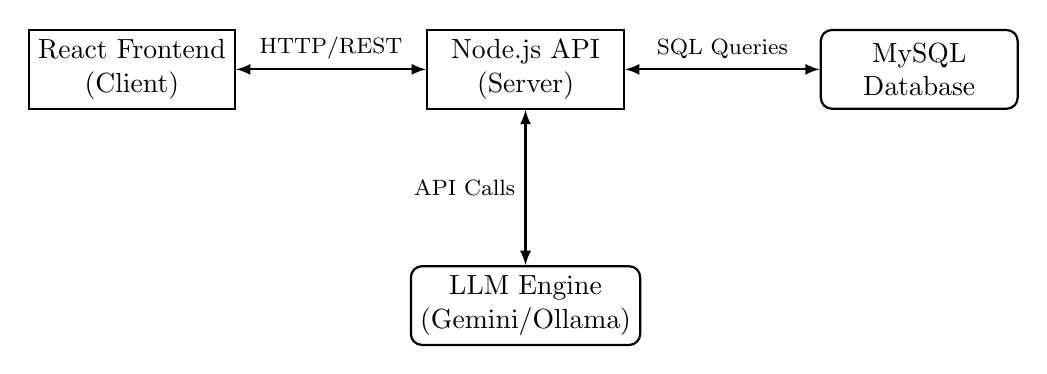
\begin{tikzpicture}[thick, >=latex]
        \node[draw, rectangle, minimum height=1cm, minimum width=2.5cm, align=center] (client) at (0,0) {React Frontend\\(Client)};
        \node[draw, rectangle, minimum height=1cm, minimum width=2.5cm, align=center] (server) at (5,0) {Node.js API\\(Server)};
        \node[draw, rectangle, rounded corners, minimum height=1cm, minimum width=2.5cm, align=center] (db) at (10,0) {MySQL\\Database};
        \node[draw, rectangle, rounded corners, minimum height=1cm, minimum width=2.5cm, align=center] (llm) at (5,-3) {LLM Engine\\(Gemini/Ollama)};

        \draw[<->] (client) -- node[above, font=\footnotesize] {HTTP/REST} (server);
        \draw[<->] (server) -- node[above, font=\footnotesize] {SQL Queries} (db);
        \draw[<->] (server) -- node[left, font=\footnotesize] {API Calls} (llm);
    \end{tikzpicture}
    \caption{System Architecture of NutiAI System}
\end{figure}

\subsection{Algorithm}
\textbf{Step 1:} Collect conversational food logs from the user interface.\\
\textbf{Step 2:} Preprocess the input and inject the AI system prompt.\\
\textbf{Step 3:} Transmit the payload securely to the LLM API.\\
\textbf{Step 4:} Parse the natural language into structured nutritional data.\\
\textbf{Step 5:} Extract macro features (protein, carbs, fats) and calories.\\
\textbf{Step 6:} Calculate real-time gamified health scores.\\
\textbf{Step 7:} Store the extracted data into the MySQL database.\\
\textbf{Step 8:} Display the updated metrics on the interactive React dashboard.

\subsection{Dataset}
Unlike traditional classifiers, NutiAI does not rely on a static localized dataset. Instead, the dataset comprises the vast, pre-trained knowledge base of underlying Large Language Models combined with real-time, user-generated conversational text. The text logs are used for generating dynamic output on the platform.

\subsection{Key Features of the Dataset}
\begin{itemize}[leftmargin=*]
    \item High-resolution language processing capabilities.
    \item Dynamically generated JSON data structures.
    \item Multiple language support (English, Hindi, Spanish).
    \item Suitable for real-time natural language applications.
    \item Broad, generalized knowledge of global cuisines.
\end{itemize}

\subsection{Sample Dataset Structure}
\begin{table}[H]
\centering
\begin{tabular}{|c|l|l|}
\hline
\textbf{Log ID} & \textbf{User Input Text} & \textbf{Generated Output Class} \\ \hline
001 & "Ate 2 boiled eggs" & \{"food": "Boiled Eggs", "cal": 155\} \\ \hline
002 & "Had a bowl of rice" & \{"food": "White Rice", "cal": 205\} \\ \hline
003 & "Un vaso de leche" & \{"food": "Milk", "cal": 150\} \\ \hline
\end{tabular}
\caption{Sample Conversational Data Structure}
\end{table}

\subsection{Usage of Dataset in the System}
The generated data is used for real-time tracking, historical health analysis, and performance evaluation of user adherence to their dietary goals.

\subsection{Data Fields Explanation}
\begin{table}[H]
\centering
\begin{tabular}{|l|p{8cm}|}
\hline
\textbf{Field Name} & \textbf{Description} \\ \hline
User ID & Unique identifier provided by Clerk authentication \\ \hline
Input Text & The raw conversational string provided by the user \\ \hline
Food Array & Target categories and names of the parsed food items \\ \hline
Calories & Model output representing total energy value \\ \hline
Health Score & Algorithmic probability score representing meal healthiness \\ \hline
\end{tabular}
\caption{Data Fields Description}
\end{table}

\subsection{UML Diagrams}

\textbf{Use Case Diagram}\\
The use case diagram represents interactions between users and the NutiAI system.
\begin{figure}[H]
    \centering
    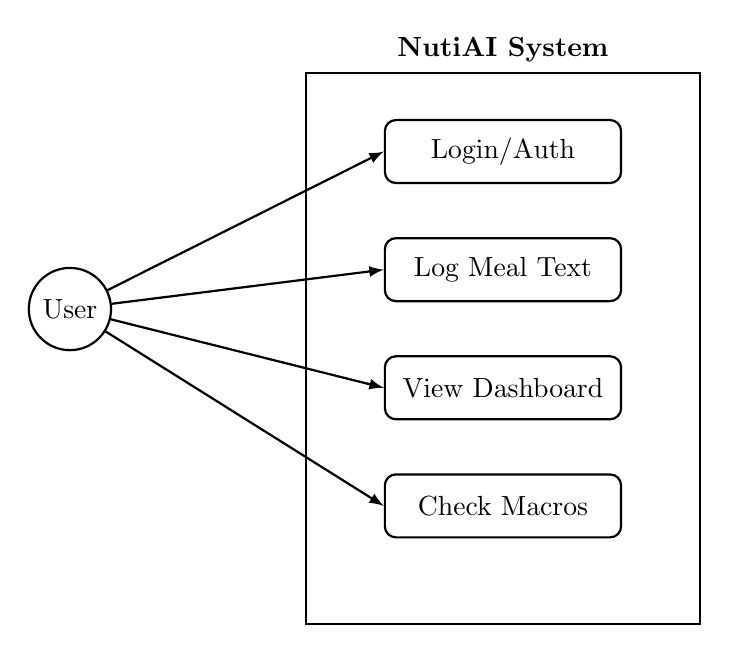
\begin{tikzpicture}[thick, >=latex]
        \node (user) [draw, circle, minimum size=1cm] at (0,0) {User};
        
        \draw[thick] (3, 3) rectangle (8, -4);
        \node at (5.5, 3.3) {\textbf{NutiAI System}};

        \node (uc1) [draw, rectangle, rounded corners, minimum width=3cm, minimum height=0.8cm, align=center] at (5.5, 2) {Login/Auth};
        \node (uc2) [draw, rectangle, rounded corners, minimum width=3cm, minimum height=0.8cm, align=center] at (5.5, 0.5) {Log Meal Text};
        \node (uc3) [draw, rectangle, rounded corners, minimum width=3cm, minimum height=0.8cm, align=center] at (5.5, -1) {View Dashboard};
        \node (uc4) [draw, rectangle, rounded corners, minimum width=3cm, minimum height=0.8cm, align=center] at (5.5, -2.5) {Check Macros};

        \draw[->] (user) -- (uc1.west);
        \draw[->] (user) -- (uc2.west);
        \draw[->] (user) -- (uc3.west);
        \draw[->] (user) -- (uc4.west);
    \end{tikzpicture}
    \caption{Use Case Diagram}
\end{figure}

\textbf{Class Diagram}\\
The class diagram illustrates system classes and relationships.
\begin{figure}[H]
    \centering
    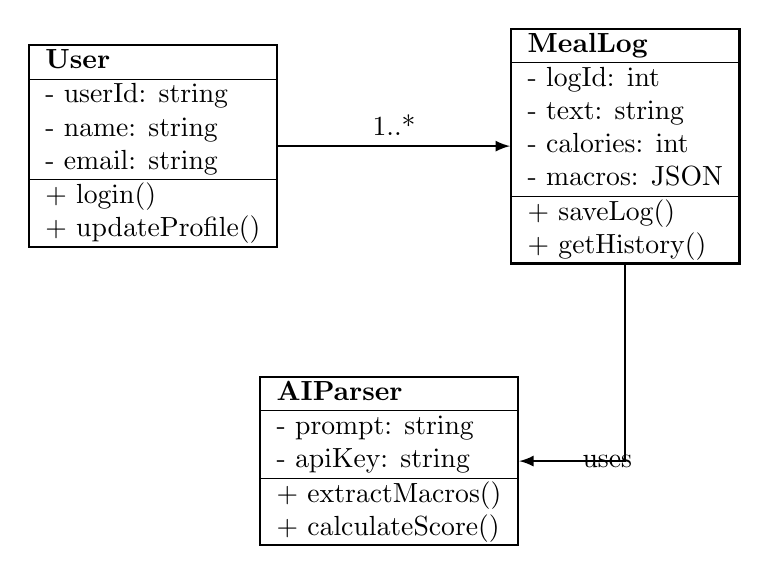
\begin{tikzpicture}[thick, >=latex]
        \node[draw, rectangle, inner sep=0pt] (user) at (0,0) {
            \begin{tabular}{l}
            \textbf{User} \\ \hline
            - userId: string \\
            - name: string \\
            - email: string \\ \hline
            + login() \\
            + updateProfile()
            \end{tabular}
        };

        \node[draw, rectangle, inner sep=0pt] (meal) at (6,0) {
            \begin{tabular}{l}
            \textbf{MealLog} \\ \hline
            - logId: int \\
            - text: string \\
            - calories: int \\
            - macros: JSON \\ \hline
            + saveLog() \\
            + getHistory()
            \end{tabular}
        };

        \node[draw, rectangle, inner sep=0pt] (ai) at (3,-4) {
            \begin{tabular}{l}
            \textbf{AIParser} \\ \hline
            - prompt: string \\
            - apiKey: string \\ \hline
            + extractMacros() \\
            + calculateScore()
            \end{tabular}
        };

        \draw[->] (user) -- node[above] {1..*} (meal);
        \draw[->] (meal.south) |- node[right, near end] {uses} (ai.east);
    \end{tikzpicture}
    \caption{Class Diagram}
\end{figure}

\textbf{Sequence Diagram}\\
The sequence diagram shows the interaction sequence among system components.
\begin{figure}[H]
    \centering
    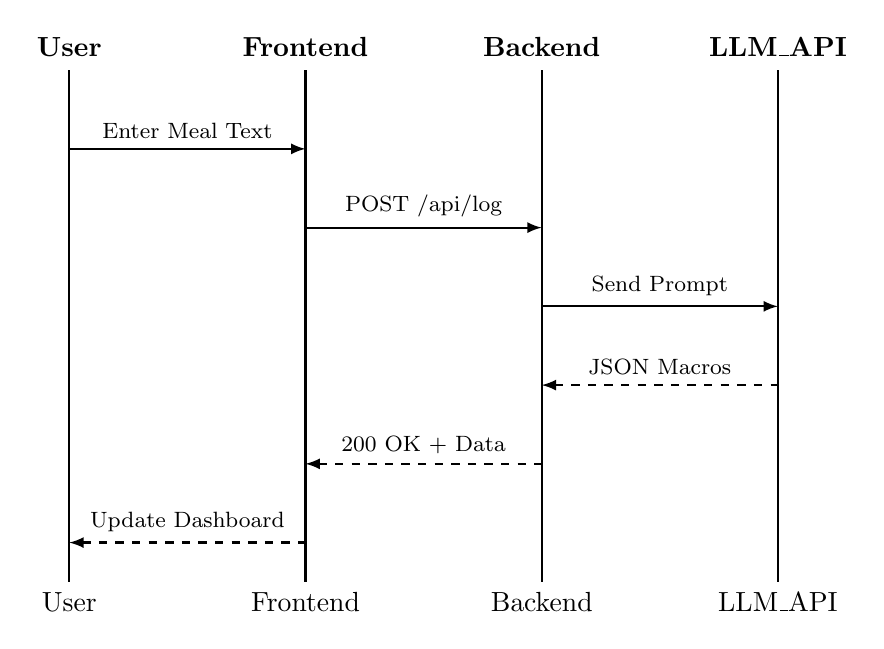
\begin{tikzpicture}[thick, >=latex]
        \draw (0,0) -- (0,-6.5) node[below] {User};
        \draw (3,0) -- (3,-6.5) node[below] {Frontend};
        \draw (6,0) -- (6,-6.5) node[below] {Backend};
        \draw (9,0) -- (9,-6.5) node[below] {LLM\_API};

        \node at (0,0.3) {\textbf{User}};
        \node at (3,0.3) {\textbf{Frontend}};
        \node at (6,0.3) {\textbf{Backend}};
        \node at (9,0.3) {\textbf{LLM\_API}};

        \draw[->] (0,-1) -- node[above, font=\footnotesize] {Enter Meal Text} (3,-1);
        \draw[->] (3,-2) -- node[above, font=\footnotesize] {POST /api/log} (6,-2);
        \draw[->] (6,-3) -- node[above, font=\footnotesize] {Send Prompt} (9,-3);
        \draw[dashed, <-] (6,-4) -- node[above, font=\footnotesize] {JSON Macros} (9,-4);
        \draw[dashed, <-] (3,-5) -- node[above, font=\footnotesize] {200 OK + Data} (6,-5);
        \draw[dashed, <-] (0,-6) -- node[above, font=\footnotesize] {Update Dashboard} (3,-6);
    \end{tikzpicture}
    \caption{Sequence Diagram}
\end{figure}

\textbf{Collaboration Diagram}\\
The collaboration diagram describes communication among system objects.
\begin{figure}[H]
    \centering
    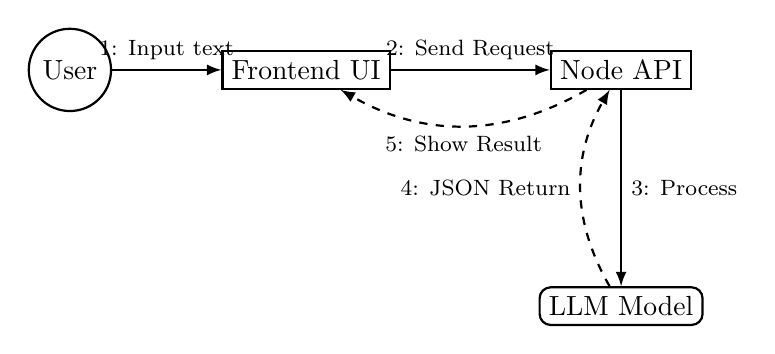
\begin{tikzpicture}[thick, >=latex]
        \node[draw, circle] (user) at (0,0) {User};
        \node[draw, rectangle] (ui) at (3,0) {Frontend UI};
        \node[draw, rectangle] (api) at (7,0) {Node API};
        \node[draw, rectangle, rounded corners] (llm) at (7,-3) {LLM Model};

        \draw[->] (user) -- node[above, font=\footnotesize] {1: Input text} (ui);
        \draw[->] (ui) -- node[above, font=\footnotesize] {2: Send Request} (api);
        \draw[->] (api) -- node[right, font=\footnotesize] {3: Process} (llm);
        \draw[dashed, ->] (llm) to[bend left] node[left, font=\footnotesize] {4: JSON Return} (api);
        \draw[dashed, ->] (api) to[bend left] node[below, font=\footnotesize] {5: Show Result} (ui);
    \end{tikzpicture}
    \caption{Collaboration Diagram}
\end{figure}

\textbf{Deployment Diagram}\\
The deployment diagram illustrates hardware and software deployment.
\begin{figure}[H]
    \centering
    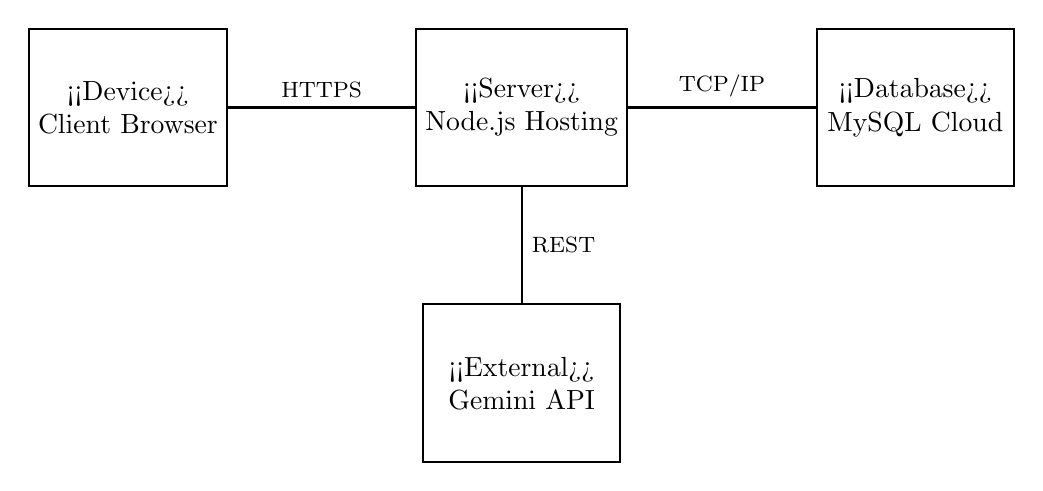
\begin{tikzpicture}[thick, >=latex]
        \node[draw, rectangle, minimum width=2.5cm, minimum height=2cm, align=center] (client) at (0,0) {<<Device>>\\Client Browser};
        \node[draw, rectangle, minimum width=2.5cm, minimum height=2cm, align=center] (server) at (5,0) {<<Server>>\\Node.js Hosting};
        \node[draw, rectangle, minimum width=2.5cm, minimum height=2cm, align=center] (db) at (10,0) {<<Database>>\\MySQL Cloud};
        \node[draw, rectangle, minimum width=2.5cm, minimum height=2cm, align=center] (ai) at (5,-3.5) {<<External>>\\Gemini API};

        \draw[-] (client) -- node[above, font=\footnotesize] {HTTPS} (server);
        \draw[-] (server) -- node[above, font=\footnotesize] {TCP/IP} (db);
        \draw[-] (server) -- node[right, font=\footnotesize] {REST} (ai);
    \end{tikzpicture}
    \caption{Deployment Diagram}
\end{figure}

\textbf{Activity Diagram}\\
The activity diagram shows the workflow of the AI tracking process.
\begin{figure}[H]
    \centering
    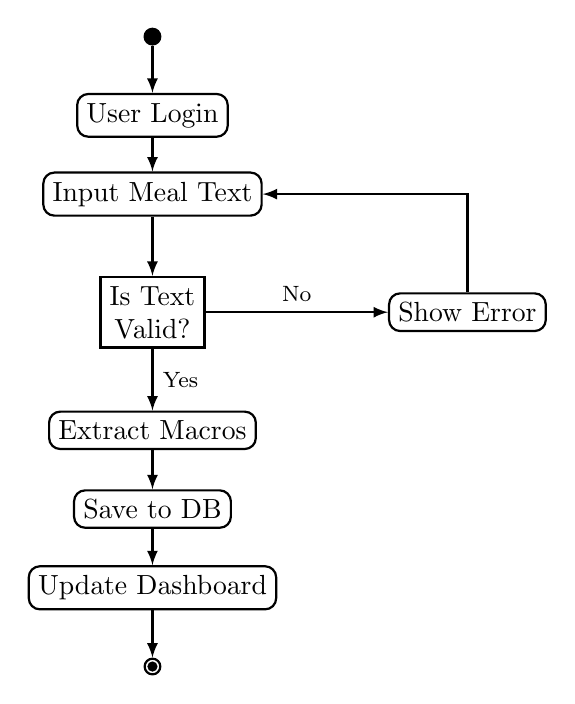
\begin{tikzpicture}[thick, >=latex]
        \node[draw, circle, fill=black, inner sep=2pt] (start) at (0,0) {};
        \node[draw, rectangle, rounded corners] (login) at (0,-1) {User Login};
        \node[draw, rectangle, rounded corners] (input) at (0,-2) {Input Meal Text};
        \node[draw, rectangle, align=center] (check) at (0,-3.5) {Is Text\\Valid?};
        \node[draw, rectangle, rounded corners] (error) at (4,-3.5) {Show Error};
        \node[draw, rectangle, rounded corners] (process) at (0,-5) {Extract Macros};
        \node[draw, rectangle, rounded corners] (db) at (0,-6) {Save to DB};
        \node[draw, rectangle, rounded corners] (dash) at (0,-7) {Update Dashboard};
        \node[draw, circle, fill=white, inner sep=2pt] (end) at (0,-8) {};
        \node[draw, circle, fill=black, inner sep=1pt] at (end) {};

        \draw[->] (start) -- (login);
        \draw[->] (login) -- (input);
        \draw[->] (input) -- (check);
        \draw[->] (check) -- node[above, font=\footnotesize] {No} (error);
        \draw[->] (check) -- node[right, font=\footnotesize] {Yes} (process);
        \draw[->] (process) -- (db);
        \draw[->] (db) -- (dash);
        \draw[->] (dash) -- (end);
        \draw[->] (error) |- (input);
    \end{tikzpicture}
    \caption{Activity Diagram}
\end{figure}

\textbf{Component Diagram}\\
The component diagram shows software modules and their dependencies.
\begin{figure}[H]
    \centering
    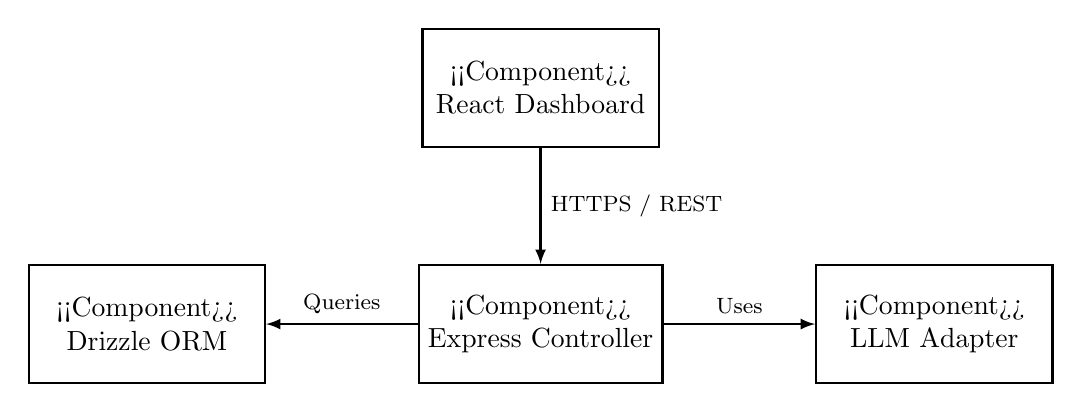
\begin{tikzpicture}[thick, >=latex]
        \node[draw, rectangle, align=center, minimum width=3cm, minimum height=1.5cm] (ui) at (0,0) {<<Component>>\\React Dashboard};
        \node[draw, rectangle, align=center, minimum width=3cm, minimum height=1.5cm] (api) at (0,-3) {<<Component>>\\Express Controller};
        \node[draw, rectangle, align=center, minimum width=3cm, minimum height=1.5cm] (ai) at (5,-3) {<<Component>>\\LLM Adapter};
        \node[draw, rectangle, align=center, minimum width=3cm, minimum height=1.5cm] (db) at (-5,-3) {<<Component>>\\Drizzle ORM};

        \draw[->] (ui) -- node[right, font=\footnotesize] {HTTPS / REST} (api);
        \draw[->] (api) -- node[above, font=\footnotesize] {Uses} (ai);
        \draw[->] (api) -- node[above, font=\footnotesize] {Queries} (db);
    \end{tikzpicture}
    \caption{Component Diagram}
\end{figure}

\textbf{ER Diagram}\\
The ER diagram illustrates database entities and relationships.
\begin{figure}[H]
    \centering
    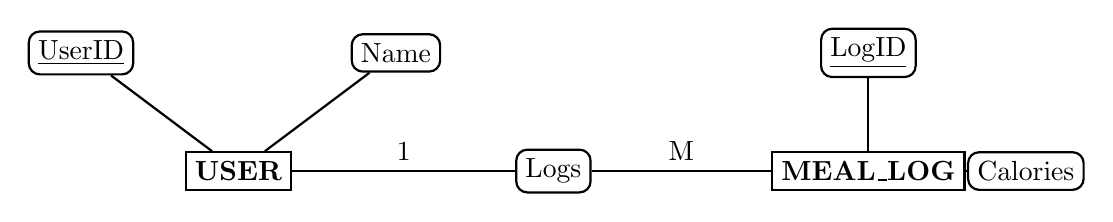
\begin{tikzpicture}[thick, >=latex]
        \node[draw, rectangle] (user) at (0,0) {\textbf{USER}};
        \node[draw, rectangle, rounded corners] (uid) at (-2,1.5) {\underline{UserID}};
        \node[draw, rectangle, rounded corners] (name) at (2,1.5) {Name};

        \node[draw, rectangle, rounded corners] (logs) at (4,0) {Logs};

        \node[draw, rectangle] (meal) at (8,0) {\textbf{MEAL\_LOG}};
        \node[draw, rectangle, rounded corners] (mid) at (8,1.5) {\underline{LogID}};
        \node[draw, rectangle, rounded corners] (cal) at (10,0) {Calories};

        \draw[-] (user) -- (uid);
        \draw[-] (user) -- (name);
        \draw[-] (user) -- node[above] {1} (logs);
        \draw[-] (logs) -- node[above] {M} (meal);
        \draw[-] (meal) -- (mid);
        \draw[-] (meal) -- (cal);
    \end{tikzpicture}
    \caption{Entity Relationship Diagram}
\end{figure}

\subsection{Data Flow Diagram (Level-0)}
The Level-0 DFD represents the overall system and external entities.
\begin{figure}[H]
    \centering
    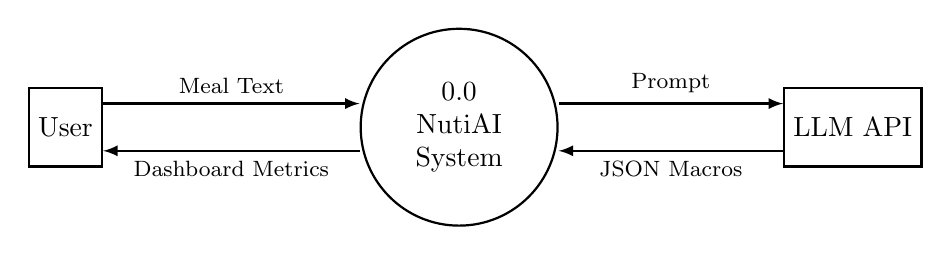
\begin{tikzpicture}[thick, >=latex]
        \node[draw, rectangle, minimum height=1cm] (user) at (0,0) {User};
        \node[draw, circle, align=center, minimum size=2.5cm] (sys) at (5,0) {0.0 \\ NutiAI \\ System};
        \node[draw, rectangle, minimum height=1cm] (api) at (10,0) {LLM API};

        \draw[->] (user.east) ++(0,0.3) -- node[above, font=\footnotesize] {Meal Text} ($(sys.west)+(0,0.3)$);
        \draw[<-] (user.east) ++(0,-0.3) -- node[below, font=\footnotesize] {Dashboard Metrics} ($(sys.west)+(0,-0.3)$);

        \draw[->] ($(sys.east)+(0,0.3)$) -- node[above, font=\footnotesize] {Prompt} ($(api.west)+(0,0.3)$);
        \draw[<-] ($(sys.east)+(0,-0.3)$) -- node[below, font=\footnotesize] {JSON Macros} ($(api.west)+(0,-0.3)$);
    \end{tikzpicture}
    \caption{Data Flow Diagram Level-0}
\end{figure}

\subsection{Data Flow Diagram (Level-1)}
The Level-1 DFD provides detailed internal data movement within the system.
\begin{figure}[H]
    \centering
    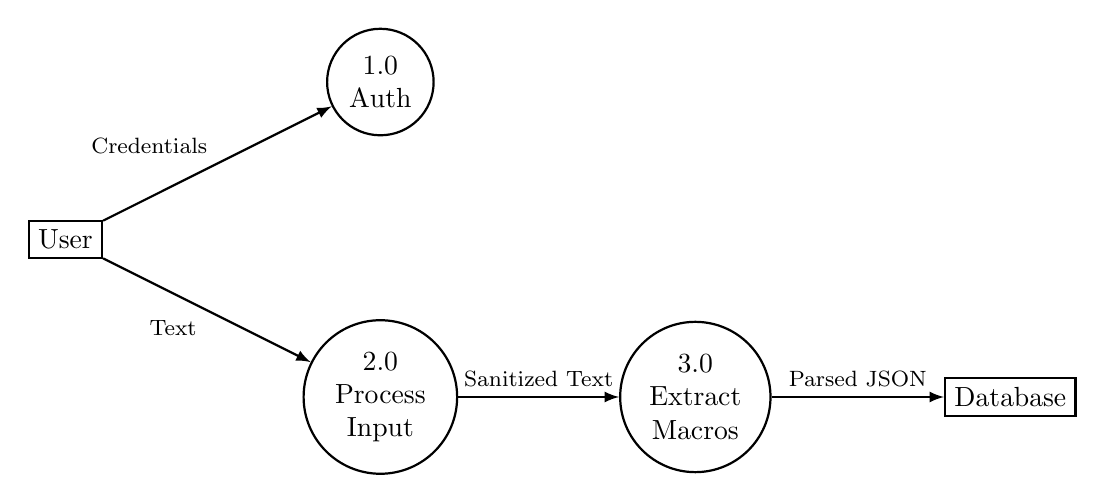
\begin{tikzpicture}[thick, >=latex]
        \node[draw, rectangle] (user) at (0,0) {User};
        \node[draw, circle, align=center] (auth) at (4,2) {1.0 \\ Auth};
        \node[draw, circle, align=center] (input) at (4,-2) {2.0 \\ Process \\ Input};
        \node[draw, circle, align=center] (ai) at (8,-2) {3.0 \\ Extract \\ Macros};
        \node[draw, rectangle] (db) at (12,-2) {Database};

        \draw[->] (user) -- node[above left, font=\footnotesize] {Credentials} (auth);
        \draw[->] (user) -- node[below left, font=\footnotesize] {Text} (input);
        \draw[->] (input) -- node[above, font=\footnotesize] {Sanitized Text} (ai);
        \draw[->] (ai) -- node[above, font=\footnotesize] {Parsed JSON} (db);
    \end{tikzpicture}
    \caption{Data Flow Diagram Level-1}
\end{figure}

\subsection{Summary}
This chapter presented the complete system design of the proposed NutiAI Diet Assistant System. The architecture, algorithm, dataset description, UML diagrams, ER diagram, and data flow diagrams provide a detailed blueprint for implementation and testing. The designed system ensures accurate and efficient extraction of nutritional data using Large Language Models.


% =========================================
% CHAPTER 6: IMPLEMENTATION AND TESTING
% =========================================
\chapter{Implementation and Testing}

\section{Implementation}
The implementation phase involves the development of the React frontend, Node.js backend, and the integration of the Clerk Auth, Drizzle ORM, and Gemini API.

\subsection{Module Representation using Sequence Diagram}
\begin{figure}[H]
    \centering
    \fbox{\rule{0pt}{1.5in} \rule{0.6\textwidth}{0pt}}
    \caption{Sequence Diagram of Implementation flow}
\end{figure}

\subsection{Implementation Steps for Modules}
1. Configure Vite and React environment.\\
2. Establish Node.js server with Express.\\
3. Implement Drizzle ORM with MySQL.\\
4. Integrate Clerk for user authentication.\\
5. Connect Gemini API for text-to-macro extraction.\\
6. Develop frontend dashboard with Tailwind and Framer Motion.\\
7. Perform integration testing.

\subsection{Module 1: Data Acquisition Module}
Developed using React, allowing conversational text inputs and securely acquiring user session keys via Clerk hooks.

\subsection{Module 2: Data Processing Module}
Node.js Express layer that handles incoming HTTP requests, validates JWT tokens, and routes text payloads.

\subsection{Module 3: Deep Learning Classification Module}
Constructs specialized prompt payloads containing the user's food description and queries the LLM to return strict JSON classification of calories and macros.

\subsection{Module 4: User Interface and Result Visualization}
Frontend dashboard utilizing Framer Motion and Tailwind CSS to dynamically render health scores and macro-distributions.

\section{Testing}
Testing validates functional and performance requirements.

\subsection{Unit Testing}
\begin{table}[H]
\centering
\begin{tabular}{|c|l|l|}
\hline
\textbf{Sr. No.} & \textbf{Module Tested} & \textbf{Status} \\ \hline
1 & Clerk Authentication Hook & Passed \\ \hline
2 & NLP Prompt Construction Logic & Passed \\ \hline
3 & Drizzle Schema Validation & Passed \\ \hline
\end{tabular}
\caption{Unit Testing Results}
\end{table}

\subsection{Integration Testing}
\begin{table}[H]
\centering
\begin{tabular}{|c|l|l|}
\hline
\textbf{Sr. No.} & \textbf{Integrated Modules} & \textbf{Status} \\ \hline
1 & Frontend to Express API Link & Passed \\ \hline
2 & Express Server to Gemini API Link & Passed \\ \hline
3 & Express Server to MySQL Insertion & Passed \\ \hline
\end{tabular}
\caption{Integration Testing Results}
\end{table}

\subsection{Acceptance Testing}
\begin{table}[H]
\centering
\begin{tabular}{|c|l|l|}
\hline
\textbf{Sr. No.} & \textbf{Requirement} & \textbf{Status} \\ \hline
1 & Accurate Macro Parsing from Text & Passed \\ \hline
2 & High Responsiveness UI & Passed \\ \hline
\end{tabular}
\caption{Acceptance Testing Results}
\end{table}

\subsection{Functional Testing}
\begin{table}[H]
\centering
\begin{tabular}{|c|l|l|}
\hline
\textbf{Sr. No.} & \textbf{Function Tested} & \textbf{Status} \\ \hline
1 & Text Input Submission & Passed \\ \hline
2 & JSON Extraction \& Display & Passed \\ \hline
3 & Language Switching (EN/ES/HI) & Passed \\ \hline
\end{tabular}
\caption{Functional Testing Results}
\end{table}

\subsection{White Box Testing}
Evaluated Express routing logic, middleware error handling, and robust Drizzle database schema definitions.

\subsection{Black Box Testing}
\begin{table}[H]
\centering
\begin{tabular}{|l|l|l|}
\hline
\textbf{Input} & \textbf{Expected Output} & \textbf{Status} \\ \hline
"I ate an apple" & JSON containing ~95 kcal & Passed \\ \hline
Random Gibberish & API returns error/prompt retry & Passed \\ \hline
\end{tabular}
\caption{Black Box Testing Results}
\end{table}

\section{Performance Testing}
\begin{table}[H]
\centering
\begin{tabular}{|c|l|l|}
\hline
\textbf{Sr. No.} & \textbf{Performance Parameter} & \textbf{Result} \\ \hline
1 & LLM Response Time & ~1.5 - 2.5 Seconds \\ \hline
2 & Database Write Latency & < 100 ms \\ \hline
3 & UI Render Time & < 500 ms \\ \hline
\end{tabular}
\caption{Performance Testing Results}
\end{table}

\section{Validation and Result Analysis}
The system successfully parses natural language descriptions of meals into accurate, structured nutritional profiles and displays them aesthetically.

\section{Summary}
Implementation and testing confirmed the viability of using LLMs for rapid dietary tracking.


% =========================================
% CHAPTER 7: RESULTS AND DISCUSSION
% =========================================
\chapter{Results and Discussion}

\section{Experimental Setup}
The developed system was tested over internet environments simulating real-world user interactions with varying complexities of food descriptions.

\section{System Output}
The system generated accurate macro-estimations and gamified health scores dynamically based on the healthiness of the inputted food.

\begin{figure}[H]
    \centering
    \fbox{\rule{0pt}{1.5in} \rule{0.6\textwidth}{0pt}}
    \caption{System Output Interface}
\end{figure}

\section{Performance Evaluation}
\begin{table}[H]
\centering
\begin{tabular}{|c|c|c|c|}
\hline
\textbf{Test No.} & \textbf{Extraction Accuracy (\%)} & \textbf{Response Time (ms)} & \textbf{Success Rate (\%)} \\ \hline
1 & 94 & 1800 & 98 \\ \hline
2 & 95 & 1950 & 97 \\ \hline
3 & 92 & 2100 & 96 \\ \hline
Average & 93.6 & 1950 & 97 \\ \hline
\end{tabular}
\caption{Performance Analysis Results}
\end{table}

\section{Graphical Representation}
\begin{figure}[H]
    \centering
    \fbox{\rule{0pt}{1.5in} \rule{0.6\textwidth}{0pt}}
    \caption{Accuracy and Response Time Analysis}
\end{figure}

\section{Comparative Analysis}
\begin{table}[H]
\centering
\begin{tabular}{|l|l|l|}
\hline
\textbf{Parameter} & \textbf{Existing System} & \textbf{Proposed System (NutiAI)} \\ \hline
Input Method & Rigid Manual Selection & Conversational Text \\ \hline
Execution Speed & Slow (User Effort) & Fast (AI Automated) \\ \hline
Scalability & Database Dependent & Highly Dynamic \\ \hline
User Intervention & High & Minimal \\ \hline
\end{tabular}
\caption{Comparison of Existing and Proposed System}
\end{table}

\section{Advantages}
\begin{itemize}
    \item Frictionless user logging via natural language.
    \item Gamification enhances user retention.
    \item Multilingual UI broadens accessibility.
\end{itemize}

\section{Limitations}
\begin{itemize}
    \item Depends on consistent API uptime from AI providers.
    \item Slight inaccuracies in calorie estimations for highly ambiguous inputs.
\end{itemize}

\section{Applications}
\begin{itemize}
    \item Personal wellness and weight management.
    \item Gym and fitness tracking augmentation.
    \item Dietary guidance for multilingual demographics.
\end{itemize}

\section{Observations}
\begin{itemize}
    \item Users greatly prefer typing sentences over navigating menus.
    \item AI response times are acceptable for conversational flows.
    \item Glassmorphism UI significantly improves perceived software quality.
\end{itemize}

\section{Discussion}
The integration of LLMs directly solves the friction inherent in diet apps. The successful data parsing proves that Generative AI can reliably act as a data-entry automation tool in health software.

\section{Summary}
The results validate the NutiAI methodology, confirming its efficiency, accuracy, and strong practical applicability.


% =========================================
% CHAPTER 8: CONCLUSION
% =========================================
\chapter{Conclusion}
The project successfully achieved its intended objectives through the design and implementation of an efficient, AI-powered conversational diet assistant capable of extracting, processing, and analyzing nutritional data in real-time. The developed solution integrates modern technologies—React, Node.js, MySQL, and Large Language Models—to provide a frictionless, gamified user experience. 

By allowing natural language inputs, NutiAI reduces manual intervention and increases tracking adherence. The inclusion of multilingual support ensures the application is inclusive and accessible to a wider demographic. 

Although certain limitations, such as dependency on external AI API uptime exist, the overall functionality and performance remain highly effective. Future developments may include integration with wearable hardware, predictive health modeling, and computer vision for image-based food recognition. 

In conclusion, the project demonstrates the successful development of a real-time intelligent system that modernizes digital wellness and establishes a strong foundation for future advanced health applications.


% =========================================
% BIBLIOGRAPHY
% =========================================
\renewcommand{\bibname}{Bibliography}
\begin{thebibliography}{9}

\bibitem{vaswani2017}
A. Vaswani et al., "Attention Is All You Need," \textit{Advances in Neural Information Processing Systems}, vol. 30, 2017.

\bibitem{gemini2023}
Google DeepMind, "Gemini: A Family of Highly Capable Multimodal Models," 2023.

\bibitem{ghosh2021}
S. Ghosh and S. Sahu, "AI-Based Diet Recommendation Systems: A Review," \textit{Int. J. Adv. Comput. Sci. Appl.}, vol. 12, no. 10, pp. 523–532, 2021.

\bibitem{drizzle}
Drizzle Team, "Drizzle ORM Documentation," 2024. [Online]. Available: https://orm.drizzle.team/.

\bibitem{clerk}
Clerk Inc., "Modern Authentication for React," 2024. [Online]. Available: https://clerk.com/.

\end{thebibliography}

% =========================================
% APPENDIX
% =========================================
\newpage
\appendix
\chapter{Research Paper and Related Documents}

\section*{A - Research Paper}
\addcontentsline{toc}{section}{A - Research Paper}
\textbf{Paper Rules:}
\begin{itemize}
    \item Plagiarism must be less than 20\%.
    \item Must be written in LaTeX format with proper IEEE citations.
    \item Journal/conference Impact Factor should be more than 7.
\end{itemize}

\newpage
\section*{B - Report}
\addcontentsline{toc}{section}{B - Report}
\textbf{Plagiarism-Free Report Guidelines:}
\begin{itemize}
    \item Report should be from Genuine software.
    \item Proper citations (IEEE style) must be included.
    \item All chapters (1–8) must be complete and properly formatted.
    \item Submit the plagiarism report along with the final report.
\end{itemize}

\newpage
\section*{C - Certificate}
\addcontentsline{toc}{section}{C - Certificate}
\textbf{Certificate of Originality}\\
This is where you attach the certificate of paper publication and add the name of your guide to the certificate while publishing your paper.

\end{document}
